\section{Full simulasjon}
\subsection{Oppsett}
Med simulasjonsblokkene klare og eit simuleringsvindu og vise resultat på, var vi
no klare for å starte simuering av anlegget.
Vi satte inn ventil tilbakemeldingsblokka på alle ventilar i programmet og oppretta eit
nytt CFC vindu som kopla tanksimuleringa av mottakstanken og reaktorane ilag med resten av
programmet. Vi valgte å starte med fleire små simuleringa før vi gikk over til å simulere heile reinseanlegget med full funksjonalitet.

Simulasjonen er satt opp slik at tilstrøymning til anlegget kan stillast av ein glidar.
Dersom ein av reaktorane er i innpumpings sekvens simulerast vi flytting av avlaupsvatn
basert på pumpekurver og løftehøgder.

Reaktortilstand er representert ved ein teksvariabel og
dei aktuelle tidsparameterane, som eksempelvis tid på reaksjonssekvensar,
er redusert for å akselerere simuleringen.

Vi har også lagt til ein alarmlogg for alle moglege alarmar anlegget kan generere, 
uavhengig om dei er aktuelle å ha med i sluttprogrammet eller ikkje.
Dette gjer oss verdifull innsikt i alle eventuelle feil som genererast og korleis programmet fungera.

\thispagestyle{fancy}
\begin{figure}[htbp]
    \centering
    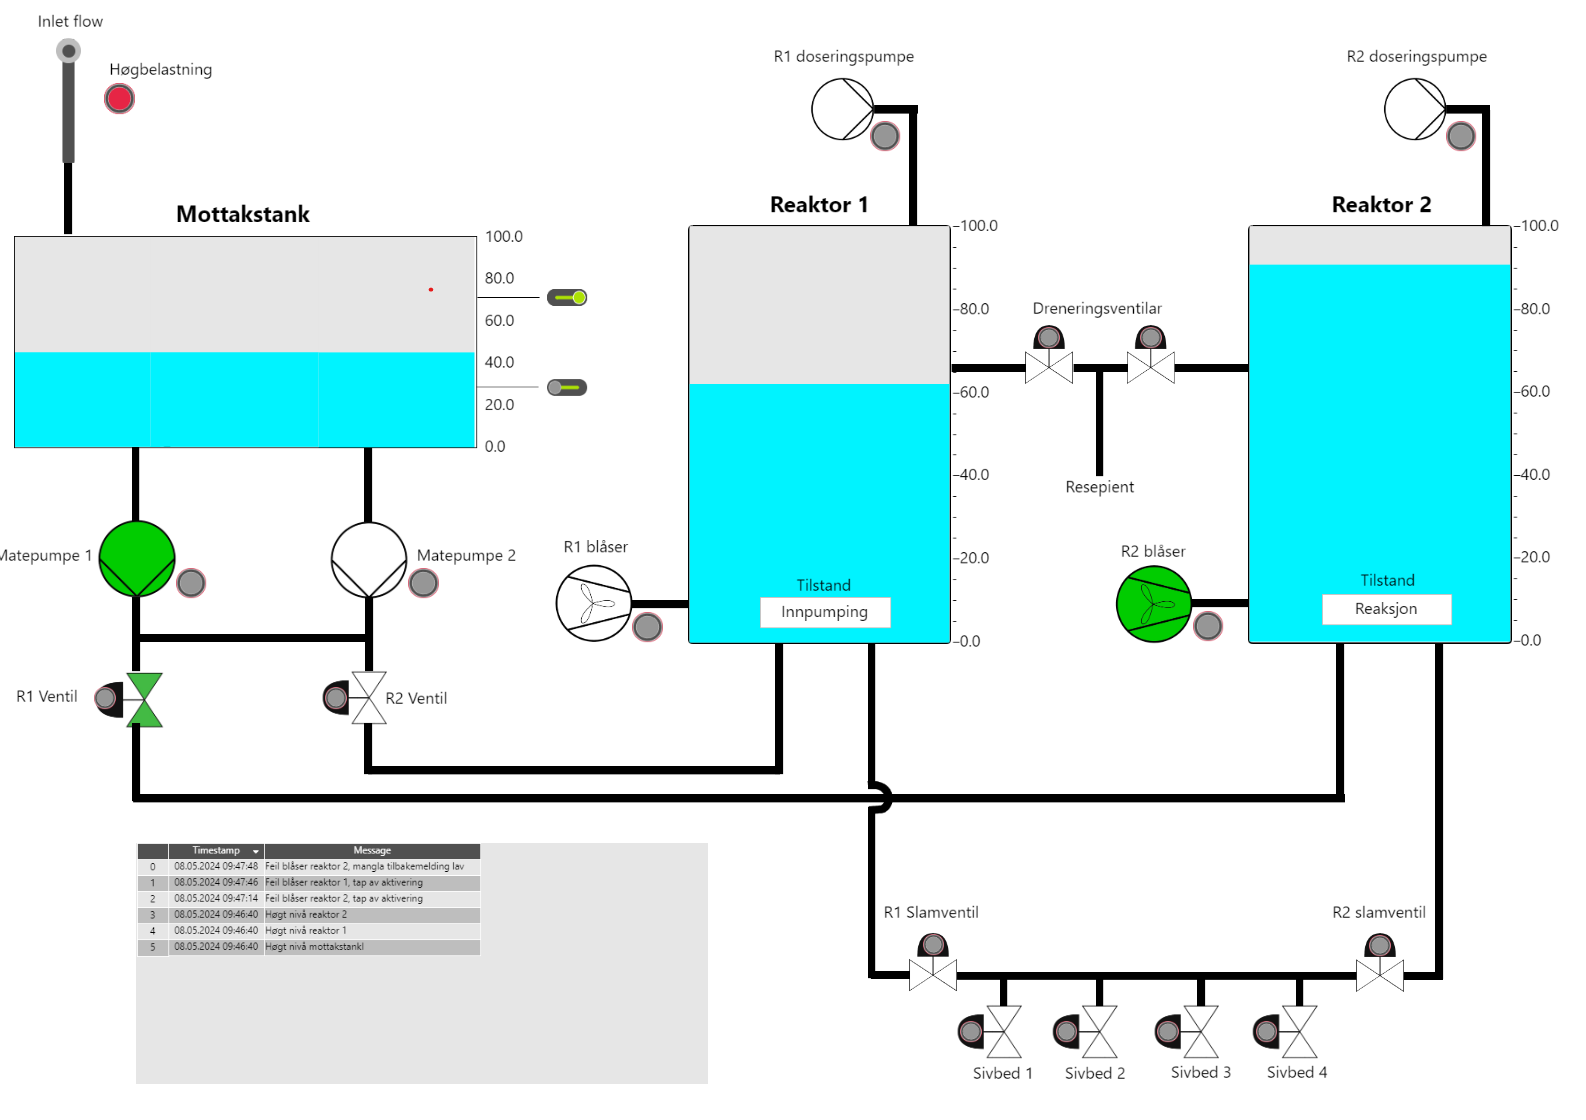
\includegraphics[scale=0.45]{Bilder/Simuleringsbilde.png}
    \caption{Oppsett av simuleringsvindu}\label{fig:Simulering}
\end{figure}

\newpage

\subsection{Resultat}

Det kom som forventa at det dukka opp avvik og 'bugs' når vi begynte å simulere.
Nokre av desse var av mindre betydning og blei utbetra undervegs i prosessen, som eksempel fungerte ikkje den tiltenkte
reaktorforriglinga på overgang frå pause til innpumpingssekvens. \newline
Andre avvik krevde meir arbeid og tilbakevending til koden, men problema låg oftast i skrivefeil, gløymde logiske oprasjonar,
CFC koplingar som var komt på feil plass og konfigurasjonsfeil.

Våra simulering av programmet var veldig vellykka og vi fekk samla masse verdifull informasjon frå anlegget i simulert drift. 
Den visuelle representasjonen var oversiktleg, der ein kunne sjå koden i drift, og det var enkelt å sjå kva koden gjorde og å oppdage feil. 

Vi fekk verifisert at programmet i grunn verkar som tiltenkt og at vi vidare er klar for ein større simulering 
der vi implimenterer dei resterande funskjonsblokkene og rettar oss mot ein fullskala test.


